\documentclass[addpoints, 12pt] {exam}
\usepackage{graphicx}
\usepackage{amsmath}
\bracketedpoints
\pagestyle{headandfoot}
\runningheadrule
\firstpageheader{Math 112}{Written Homework 10}{Due March 29th 2024}
\runningheader{Math 112}{ Page\; \thepage\; of\; \numpages}{Written Homework 10}
\firstpagefooter{}{}{}
\runningfooter{}{}{}
\setlength\answerskip{2ex}
\setlength\answerlinelength{1.5in}
\begin{document}

\begin{center}
\fbox{\fbox{\parbox{5.5in}{\centering
Directions:\\Please only put your final, well written solutions, in the space provided.\\ Give exact answers (simplified radicals or fractions).\\If you use additional paper clearly label the question and upload pages after the question page.\\Use complete sentences and explain your reason as much as possible.\\There are \numquestions\,  questions and \numpoints\, points total
}}}\end{center}
\vspace{0.1in}
\makebox[\textwidth]{Name:\enspace\hrulefill}
%\qformat{Question \thequestion \dotfill \thepoints}%

\begin{questions}

\question Our goal is to determine the algebraic form for a function given in the graph below. This function is a {\bf rational function} and will be in the form of: \[f(x)=\displaystyle\frac{ax+b}{cx+d}\]
\begin{center}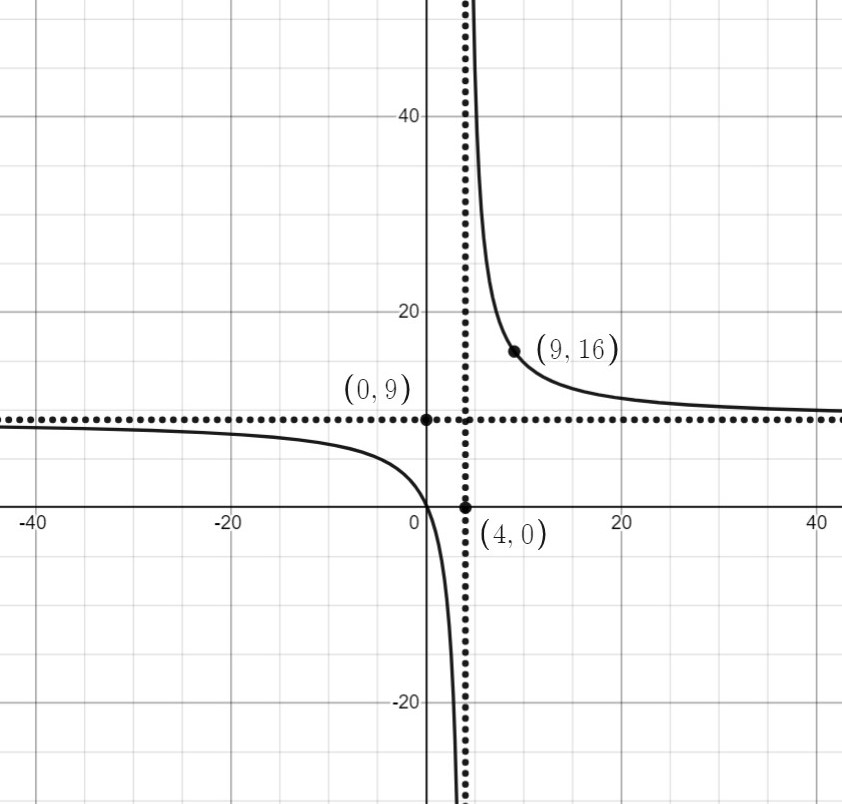
\includegraphics[scale=0.65]{HW5.1}\newline\end{center}
\begin{parts}
\part[1] Based on the graph, what is the horizontal asymptote?\answerline
% y=9 %
\part[1] Based on the {\bf formula}, what is the horizontal asymptote? Your answer will depend on some combination of the parameters \(a,b,c,\) and \(d\). \answerline
% y = a/c %
\part[2] Based on the previous two parts, pick values for \(a\) and \(c\) that give the correct horizontal asymptote.\answerline
% y = 9/1, a = 9, c = 1 (Easiest choices)%
\part[1] Based on the graph, what is the vertical asymptote? \answerline
% x= 4 %
\part[1] Using your choices for \(a\) and \(c\), what value of \(d\) will give the correct vertical asymptote?\vspace{0.25in}\answerline
% (1)*4 + d = 4 %
% d = -4 %
\part[2] Using your choices for \(a\), \(c\) and \(d\) as well as the given point \((9, 16)\), determine the value of \(b\).\vspace{0.25in}\answerline
% (9(9)+b)/(9-4) = 16 %
% (81+b)/5 = 16 %
% 81+b = 80%
% b=-1 %
\part[1] Put all your previous work together and write down the full rational function equation:\newline\newline\[f(x) = \]\vspace{0.25in}\newline
\part[1] Is this function the only possible answer? Also, explain whether or not you think the {\bf vertical intercept} is reasonable in the context of the graph.
\end{parts}
\newpage
\question For this question, we will be considering the function \[g(x) = \displaystyle\frac{x^2-25}{2x^2-4x-6}\]
\begin{parts}
\part[2] What is the {\bf domain} of this function? Please give your answer in interval notation.\vspace{0.5in}\answerline
\part[2] What are the {\bf zeros} of \(g(x)\)? \vspace{0.5in} \answerline
\part[1] If there is one, what is the {\bf horizontal asymptote}?  \newline Write DNE if it doesn't exist.\answerline
\part[2] If there are any, what are the {\bf vertical asymptote(s)}? \newline Write None if there are none. \answerline
\part[1] If it exists, what is the {\bf vertical intercept}? \newline Write DNE if it doesn't exist.\answerline
\part[2] Draw and label the graph of the function based on your findings above. Be sure to include and clearly label each of the features you found.
\end{parts}
\newpage
\question A large mixing tank currently contains 50 gallons of water. The company makes a simple syrup for use in their other products, which requires sugar to be mixed into the water. 

In addition to the water already in the tank, a tap will open that pours out 30 gallons of water per minute into the mixing tank while at the same time that sugar is poured at a rate of 3 pounds per minute from a hopper that contains 36 pounds of sugar. Large paddles spin to dissolve the sugar and form the simple syrup. 

\begin{parts}
\part[3]Let \(S(t)\) be the function representing the pounds of \emph{sugar} in the mixing tank as a function of time in minutes where \(t=0\) represents the point that the tap and sugar start. Determine the correct formula for \(S(t)\).\vspace{.5in}\answerline
\part[3]Let \(W(t)\) be the function representing the total volume of \emph{water} (in gallons) in the tank as a function of time in minutes, starting at the same time as above. Determine the correct formula for \(W(t)\).\vspace{.5in}\answerline 
\part[1] What domain is appropriate for these two functions? Give your answer in interval notation. Explain your answer.\vspace{1in}\answerline

The \textbf{concentration} of sugar in the final mixture is determined as the total sugar in the mixture divided by the total water.

\part[1] Let \(C(t)\) represent the concentration of sugar as a function of time. What is the correct formula for \(C(t)\) based on your previous answers?\vspace{0.25in}\answerline
\part[2] Using a graphing utility like Desmos or TI-84, answer the question: When is the concentration of sugar in the solution the greatest?
\end{parts}
\newpage

\question The manufacturer of the water toy ``Silly Soaker'' is rolling out a new line of toys. After research and development, they have come to a design which will incur a fixed cost of \(\$12,000\) (needed to retool the factory for the new product line) with a \(\$3.75\) cost in materials per unit made.

As part of their decision in picking a price to sell each unit at, it is common to consider the cost \emph{averaged} over all units manufactured. Let \(x\) represent the number of toys produced and \(C(x)\) represent the \emph{average cost} of the toy.
\begin{parts}
\part[3] Determine the correct formula for \(C(x)\). \vspace{0.5in}\answerline
\part[1] What is a reasonable domain for this function? Explain your answer. \vspace{0.5in}\answerline
\part[1] What is the average cost if they manufactur exactly \(10,000\) units?\answerline
\part[1] What (if any) are the \emph{vertical asymptotes} of \(C(x)\) (consider your domain!)\answerline
\part[1] What is the \emph{horizontal asymptote} of \(C(x)\)?\answerline
\part[2] Explain what a horizontal asymptote represents in a function like \(C(x)\)?\vspace{1.5in}
\part[1] Include a sketch or screenshot of your graph that shows what happens to the graph over the course of its domain (this may be a separate page).
\vspace{2.5in}

\end{parts}
\end{questions}
\end{document}